\documentclass[a4paper]{article}
\usepackage{amsmath, amsthm, amssymb, multicol,mathtools}
\usepackage[margin=0.5in]{geometry}
\usepackage{tikz}

\pagenumbering{gobble}

\begin{document}

\begin{multicols}{2}

	\section{Informal Proofs}
	Can you speak English? Great! Informal proofs involve
	proving stuff with a combination of math and English.
	Now go out there and spout bullshit.

	\section{Proofs by Induction}

	\section{Number Theory}

	\section{Set Theory}

	\section{Sequences and Series}

	\section{Combinatorics}
	\subsection{Permutations and Combinations}
	\textbf{r-permutation}: a permutation of a set using r number of
	elements.\\
	\textbf{Number of permutations}= $P(n,r)=\dfrac{n!}{(n-r)!}$\\r-permutation
	of set with n distinct elements\\
	\textbf{r-combination}: a subset of the set with r elements\\
	number of r combinations of a set with n elements is\\
	C (n, r) or
	$\binom{n}{r}=\dfrac{n!}{(n-r)!r!}$ = number of r permutations
	aka binomial coefficient\\
	\textbf{Binomial theorem}: x and y are variable n is nonneg int\\
	${(x+y)}^{n}=\sum{n}{j=0}\binom{n}{j}x^{n-j}y^{j}$\\
	\textbf{Pascal's Identity}: if n and k are ints with $n \geq k \geq 0$ then
	\\
	$\binom{n+1}{k}=\binom{n}{k-1}+\binom{n}{k}$\\
	\textbf{Permutation with reputation}: string of length r with n choices
	$n^r$\\
	if no repetition allowed $P(n,r)=\dfrac{n!}{(n-r)!}$\\
	\textbf{Combinations with repetition}: the number of r combinations from a
	set with n elements when repetition of elements is allowed is\\
	$C(n+r-1,r)=C(N+r-1,n-1)=\binom{n+r-1}{r}$\\
	\textbf{Stars and Bars}:Choose 6(r) cookies from 4(n) kinds of cookies how
	many ways to place 3 bars\\
	\textbf{Number of solutions}:$x_1+x_2+x_3=11$ where xs are non-negative
	ints\\
	\textbf{Permutations with indistinguishable Objects}: reorder SUCCESS\\
	3 S's $\binom{7}{3} 2 c's \binom{4}{2} \binom{remaining}{amount of current object}=\dfrac{n!}{n_1!n_2!\cdots n_k!}$\\
	$\binom{3-1+11}{3-1}$ (stars and bars)\\
	$\binom{r+n-1}{n-1}=\binom{9}{3}$\\
	\textbf{Division rule}: if there are n ways to do something but for any way
	2 there are (d-1) ways that are identical then there are n/d ways to do it
	\\
	\textbf{Ramsey Party Problem\\
	Ramsey Numbers}: $R (m,n)$ for m and n positive ints greater than 1 the
	minimum number of people at a party such that there are either m mutual
	friends of n mutual enemies.
	\subsection{Pigeonhole Principle}
	3 pigeons 2 holes = at least 2 pigeons in one hole\\
	$\lceil\dfrac{N}{k}\rceil$\\N pigeons and k holes

	\section{Discrete Probability}
	\subsection{Laplace's Theory or Probability}
	\subsection{Probability Distributuions}
	\subsection{Conditional Probability}
	\subsection{Bayes' Theorem}
	\subsection{Independence}
	\subsection{Random Variables and Expectation}

	\section{Models of Computation}
	\subsection{Regular Languages}
	\begin{itemize}
		\item A \textbf{languages} is any subset of $\Sigma^*$
		\item Example: $\Sigma = {a, b}$ \\
					${\lambda}$ \\
					${a, aa, aab}$ \\
					${\lambda, a, aa, aaa, aaaa, aaaaa}$ \\
		\item We say a Finite Automata accepts a string if, when it processes that
					string, it ends in an accept state.
	\end{itemize}
	\subsection{Finite Automata and Regular Expressions}
	Example of a finite automata:
	\begin{center}
		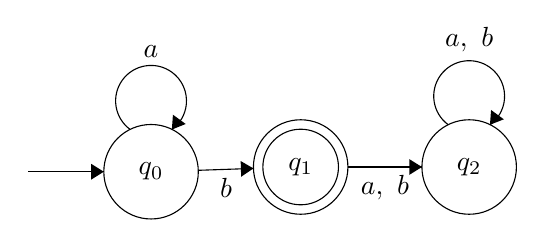
\begin{tikzpicture}[scale=0.2]
			\tikzstyle{every node}+=[inner sep=0pt]
			\draw [black] (15.1,-29.5) circle (3);
			\draw (15.1,-29.5) node {$q_0$};
			\draw [black] (24.6,-29.2) circle (3);
			\draw (24.6,-29.2) node {$q_1$};
			\draw [black] (24.6,-29.2) circle (2.4);
			\draw [black] (35.3,-29.2) circle (3);
			\draw (35.3,-29.2) node {$q_2$};
			\draw [black] (13.777,-26.82) arc (234:-54:2.25);
			\draw (15.1,-22.25) node [above] {$a$};
			\fill [black] (16.42,-26.82) -- (17.3,-26.47) -- (16.49,-25.88);
			\draw [black] (18.1,-29.41) -- (21.6,-29.29);
			\fill [black] (21.6,-29.29) -- (20.79,-28.82) -- (20.82,-29.82);
			\draw (19.87,-29.88) node [below] {$b$};
			\draw [black] (27.6,-29.2) -- (32.3,-29.2);
			\fill [black] (32.3,-29.2) -- (31.5,-28.7) -- (31.5,-29.7);
			\draw (29.95,-29.7) node [below] {$a,\mbox{ }b$};
			\draw [black] (33.977,-26.52) arc (234:-54:2.25);
			\draw (35.3,-21.95) node [above] {$a,\mbox{ }b$};
			\fill [black] (36.62,-26.52) -- (37.5,-26.17) -- (36.69,-25.58);
			\draw [black] (7.3,-29.5) -- (12.1,-29.5);
			\fill [black] (12.1,-29.5) -- (11.3,-29) -- (11.3,-30);
		\end{tikzpicture}
	\end{center}
	A machine only accepts \textbf{one} language. If it accept no strings, it
	recognizes the langauge $\o$. \\
	A palindrome is a string whose reversal is identical to the string.
	\subsection{Contex-Free Languages and Grammars}
	\begin{itemize}
		\item A \textbf{regular expression} is a way of describing a regular
					language.
		\item A grammar gives the rules for expressing a language.
		\item A \textbf{context-free} language can be described by a
					\textbf{context-free grammar}.
		\item Theorem: A language is context-free if and only if some
					(nondeterministic) pushdown automaton recognizes it.
		\item A CFG is \textbf{ambiguos} if some string $w \in L(G)$ has at least
					two different leftmost derivations.
		\item Some context-free languages habe only ambiguous grammars.
	\end{itemize}
	Example: Designe a CFG for $L(G) = \{ww^R : w \in \{a, b\}^*\}$ \\
	\begin{align*}
		S & \rightarrow aSa     \\
		S & \rightarrow bSb     \\
		S & \rightarrow \lambda \\
		S & \rightarrow a|b
	\end{align*}
	\subsection{Turning Machines}
	A turing machine:
	\begin{itemize}
		\item Reads input from tape, one character at a time.
		\item Changes state based on input.
		\item Outputs ``accept'' or ``reject'' when input ends.
	\end{itemize}
	In each step, a Turing machine \textbf{reads a symbol, writes a symbol, and
	moves left or right.} A turing machine cannot move left past the start of a
  tape, rather, it stays in place. \\
	A Turing machine has an accept stte and and a reject state. If it reaches one
	of these states, it outputs accept or rejects and stops reading input. An
	infinate loop means ``reject.'' \\

	\section{Limitations of Computational Models}
	\begin{itemize}
		\item The language consisting of all Turing Machines encodings is an
					infinate set.
		\item Not all languages are recognizeable by a Turing Machine.
		\item Infinte sets come in different sizes.
	\end{itemize}
	\subsection{Countable vs. Uncountable Sets}
	\begin{itemize}
		\item An infinite set $S$ is \textbf{countable} if and only if ther exists a
					bijective function $f: S \rightarrow Z^+$. $f$ maps each element of
					$S$ to exactly one element of $Z^+$ and every element of $Z^+$ is
					mapped by some element of $S$, under $f$.
		\item All infinite countable sets are the same size, the same size as $Z^+$.
		\item All finite sets are countable.
		\item \textbf{All subsets of countable sets are countable.}
	\end{itemize}
	\subsection{Enumerators}
	\begin{itemize}
		\item An enumerator for a langage $S$ is a Turing Machine that generates
					all the strings in $S$ one by one. Each string is generated in finite
					time.
		\item \textbf{A set is countable if we can find an enumeration procedure for
					the set.}
		\item Theorem: The set of all Turing Machines is countable.
	\end{itemize}
	\subsection{Languages}
	\begin{itemize}
		\item There are some languages not accepted by Turing Machines.
		\item These languages cannout be described by algorithms.
		\item A languages is called \textbf{Turing recognizable} if some Turing
					Machine recognizes it (aka accepts it).
		\item A language is called \textbf{Turing decidable} if some Turing machine
					decides it.
		\item Not all languages are recognizeable by a turing machine.
	\end{itemize}

	\section{Decision Problems}
	\begin{itemize}
		\item \textbf{Decision problems} are problems with a YES or NO answer.
		\item A language is \textbf{Turing-decidable} if some Turing Machine decides
					it.
		\item The Turing Machine always halts.
		\item Theorem: The membersip problem is undecidable. There is no Turing
					Machine that can decide whether $M$ accepts $w$ for all $M$ and $w$.
		\item Theorem: The halting probelm is undecidable. There is no Turing
					machine that can determine whether $M$ halts on input for $w$ for all
					$M$ and $w$ (Proved in Turing's 1936 paper).
	\end{itemize}

	\section{P and NP}
	$$P \subseteq NP$$
	\begin{itemize}
		\item Every language that can be decided by a deterministic Turing
					Machine in polynomial time can be decided by a nondeterministic
					Turing Machine in polynomial time.
		\item Every deterministic Turing Machine is a nondeterministic Turing
					Machine.
		\item Is $P = NP$? We don't know.
		\item Does the satisfiability problem have a polynomial time deterministic
					algorithm? We don't know.
		\item Cook's Theorem: The satisfiability problem is $NP$-complete.
	\end{itemize}

\end{multicols}

\end{document}
